\chapter{GitHub}
\par
\section{O que é?}
O GitHub é uma plataforma de hospedagem de código-fonte que utiliza o sistema de controle de versão Git. Ele permite que desenvolvedores colaborem em projetos, compartilhem código e gerenciem alterações de forma eficiente. Com o GitHub, é possível criar repositórios, realizar pull requests, revisar código e acompanhar o histórico de alterações.
\par
Além disso, o GitHub oferece recursos adicionais, como GitHub Pages para hospedagem de sites estáticos, GitHub Actions para automação de fluxos de trabalho e integração com diversas ferramentas de desenvolvimento.
\par
O GitHub é amplamente utilizado na indústria de software, sendo uma ferramenta essencial para desenvolvedores, equipes de desenvolvimento e organizações que buscam melhorar a colaboração e a gestão de projetos de software.
\par
\section{Criando seu perfil no GitHub}
Para criar uma conta no GitHub, siga os passos abaixo:
\begin{enumerate}
  \item Acesse o site do GitHub: \url{https://github.com/}
  \item Clique em "Sign up" no canto superior direito.
  \item Preencha os campos solicitados, como endereço de e-mail, nome de usuário e senha - Figura \ref{fig:signup_page}, p.\pageref{fig:signup_page}.
  \begin{figure}[H]
    \centering
    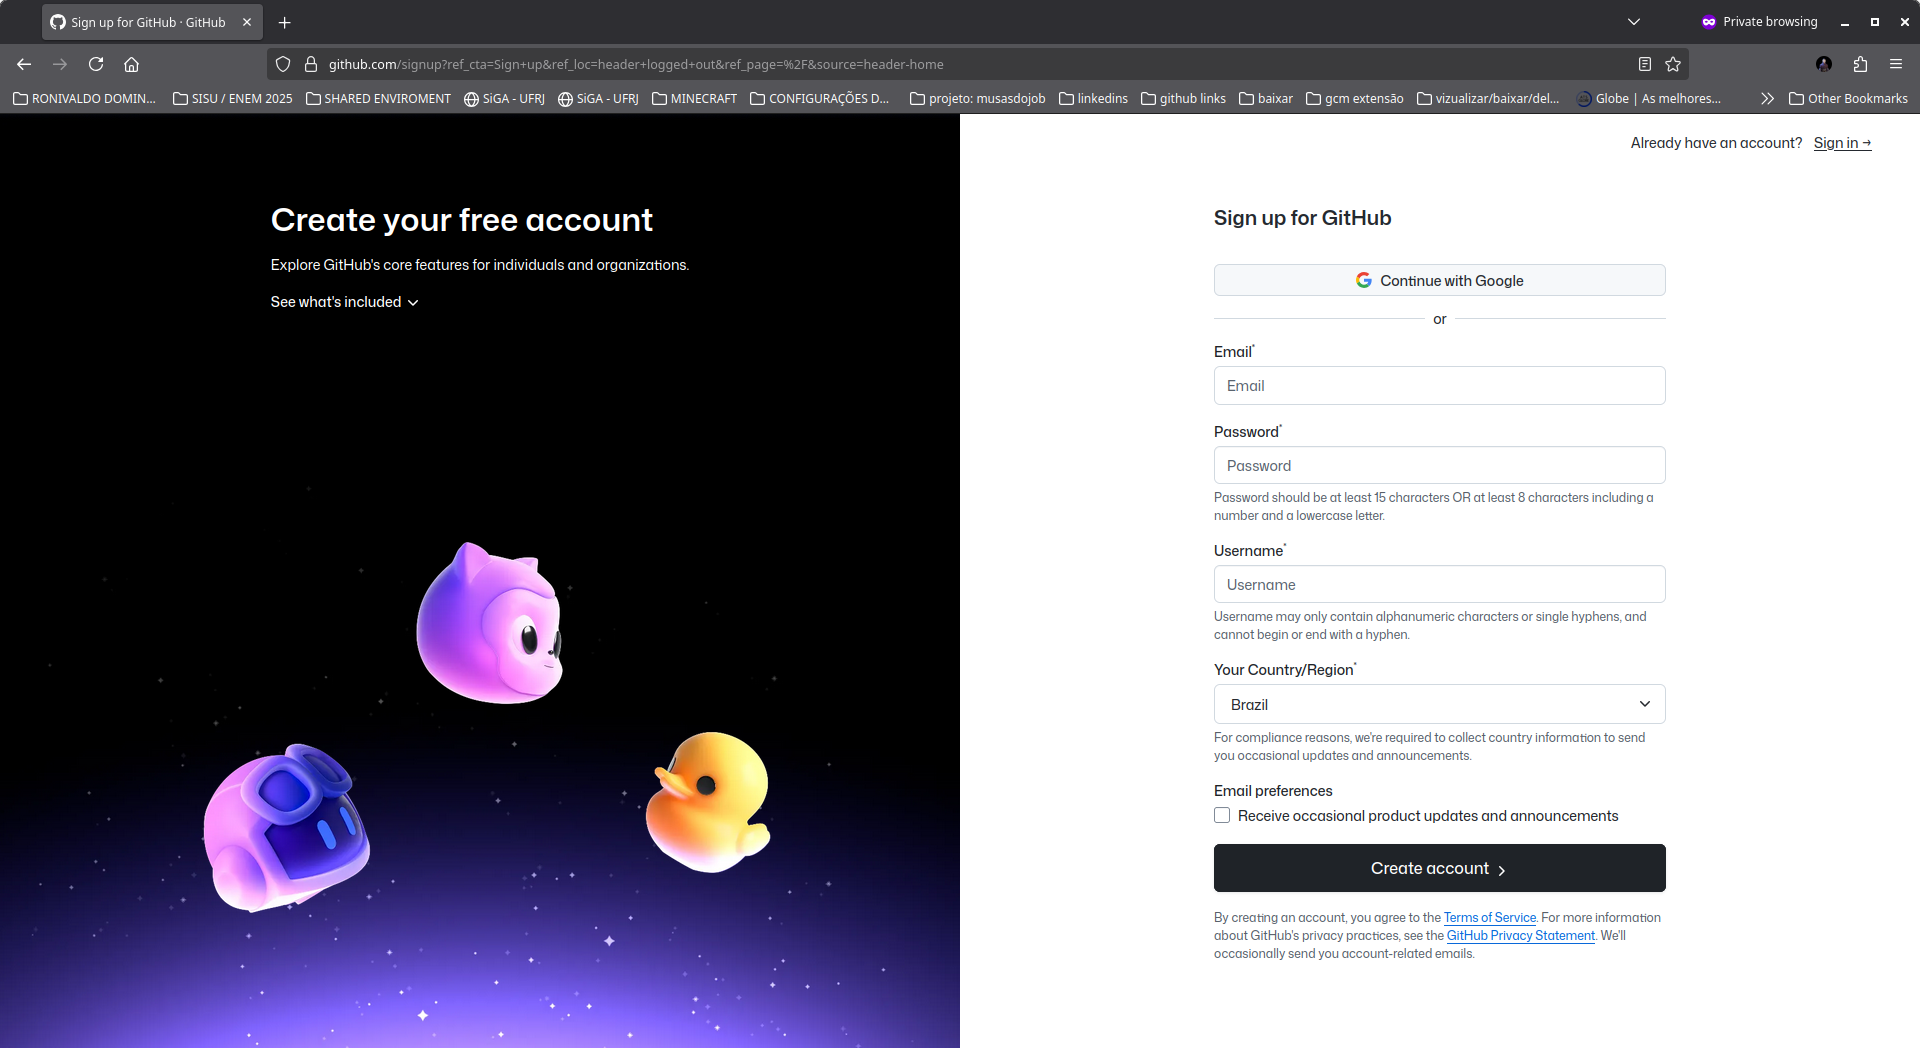
\includegraphics[width=0.8\textwidth]{./assets/images/01_signup_page.png}
    \caption{Página para a criação de conta no GitHub}
    \label{fig:signup_page}
  \end{figure}
  \item Siga as instruções na tela para concluir o processo de criação da conta.
  \item Ao final você verá a tela inicial do GitHub - Figura \ref{fig:signed_page}, p.\pageref{fig:signed_page}.
  \begin{figure}[H]
    \centering
    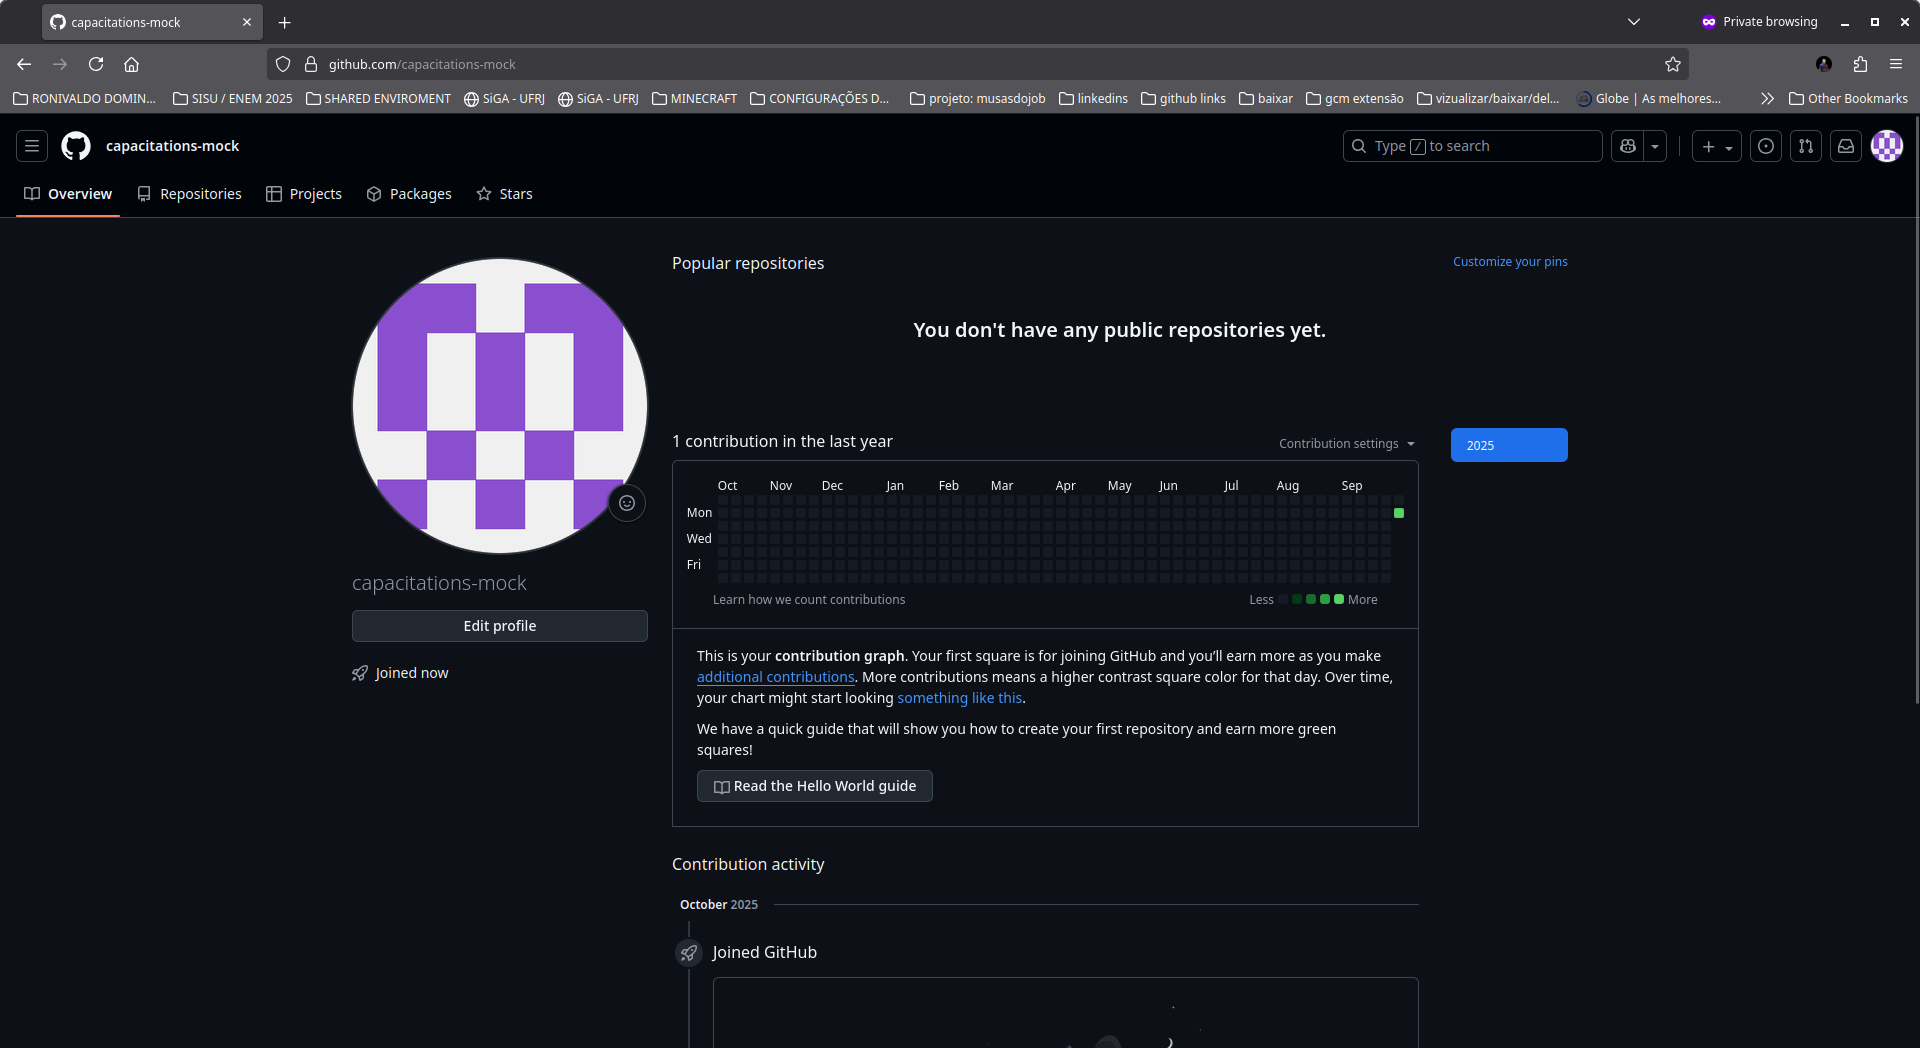
\includegraphics[width=0.8\textwidth]{./assets/images/02_signed_page.png}
    \caption{Primeira visão do GitHub depois de criar a conta}
    \label{fig:signed_page}
  \end{figure}
\end{enumerate}
\par
Após criar a conta, você poderá acessar o GitHub e começar a explorar seus recursos.
\par
\subsection{E-mail acadêmico e GitHub Student Developer Pack}
Para usar o GitHub Student Developer Pack e tornar sua conta uma GitHub Pro, você deve associar um e-mail acadêmico à sua conta. Isso pode ser feito nas configurações da conta, na seção "Emails". Adicionar um e-mail acadêmico pode ajudar a validar sua identidade como estudante ou profissional da área de tecnologia.
\par
Com isso o GitHub Student Developer Pack fornece acesso gratuito a diversas ferramentas e serviços para estudantes. Para se inscrever, você precisará verificar seu status de estudante com um e-mail acadêmico válido.
\par
\subsubsection{Por que usar o GitHub Student Developer Pack?}
O GitHub Student Developer Pack oferece uma série de benefícios, incluindo acesso gratuito a ferramentas de desenvolvimento, serviços de hospedagem e outros recursos que podem ser extremamente úteis para estudantes que estão aprendendo a programar e desenvolver software.
\par
\subsubsection{GitHub Free vs GitHub Student Developer Pack (GSDP)}
A conta gratuita do GitHub oferece recursos básicos, como repositórios públicos e privados, colaboração em projetos e integração com outras ferramentas. Já a conta GitHub Student Developer Pro oferece benefícios adicionais, como acesso a ferramentas premium, maior capacidade de armazenamento e recursos avançados de colaboração.
\par
\newpage
\subsubsection{GitHub Free vs GSDP}
\begin{table}[h!]
    \centering
    \begin{tabularx}{\textwidth}{|p{3cm}|p{3cm}|p{3cm}|X|}
        \hline
        \textbf{Recurso / Limite} & \textbf{GitHub Free (Conta Pessoal)} & \textbf{GitHub Student Developer Pack (GSDP)} & \textbf{Diferencial Estratégico} \\
        \hline
        Acesso a Repositórios Privados & Ilimitado (Recursos Limitados) & Ilimitado (Recursos Pro/Avançados) & Governança de Código \\
        \hline
        Minutos do GitHub Actions (Mensal) & 2,000 minutos & 3,000 minutos & Maior Resiliência de CI/CD (+50\%) \\
        \hline
        Armazenamento de Packages & 500 MB & 2 GB & Suporte a Artefatos e Contêineres (+400\%) \\
        \hline
        Horas de Core do Codespaces (Mensal) & 120 horas & 180 horas & Desenvolvimento em Nuvem Estendido \\
        \hline
        Armazenamento Codespaces (Mensal) & 15 GB & 20 GB & Maior Capacidade de Workspace \\
        \hline
        Revisores Obrigatórios (Private Repos) & Não Disponível & Disponível (Recurso Pro) & Enforçamento de Qualidade e Compliance \\
        \hline
        Suporte & Suporte Comunitário & Suporte Comunitário & Base de Suporte \\
        \hline
        Acesso ao GitHub Copilot & Não Incluído (Subscrição Paga) & Incluído (Geralmente Copilot Pro) & Produtividade e Aceleração por IA \\
        \hline
    \end{tabularx}
    \caption{GitHub Free (Pessoal) vs. GitHub Student Developer Pack (Pro)}
    \label{tab:core_comparison}
\end{table}
\par
\newpage
\section{Obtendo o GitHub Student Developer Pack}
\begin{enumerate}
  \item Vá até as configurações da sua conta no GitHub.
  \item Na seção "Emails", adicione seu e-mail acadêmico - Figura \ref{fig:adding_academic_email}, p.\pageref{fig:adding_academic_email}.
  \begin{figure}[H]
    \centering
    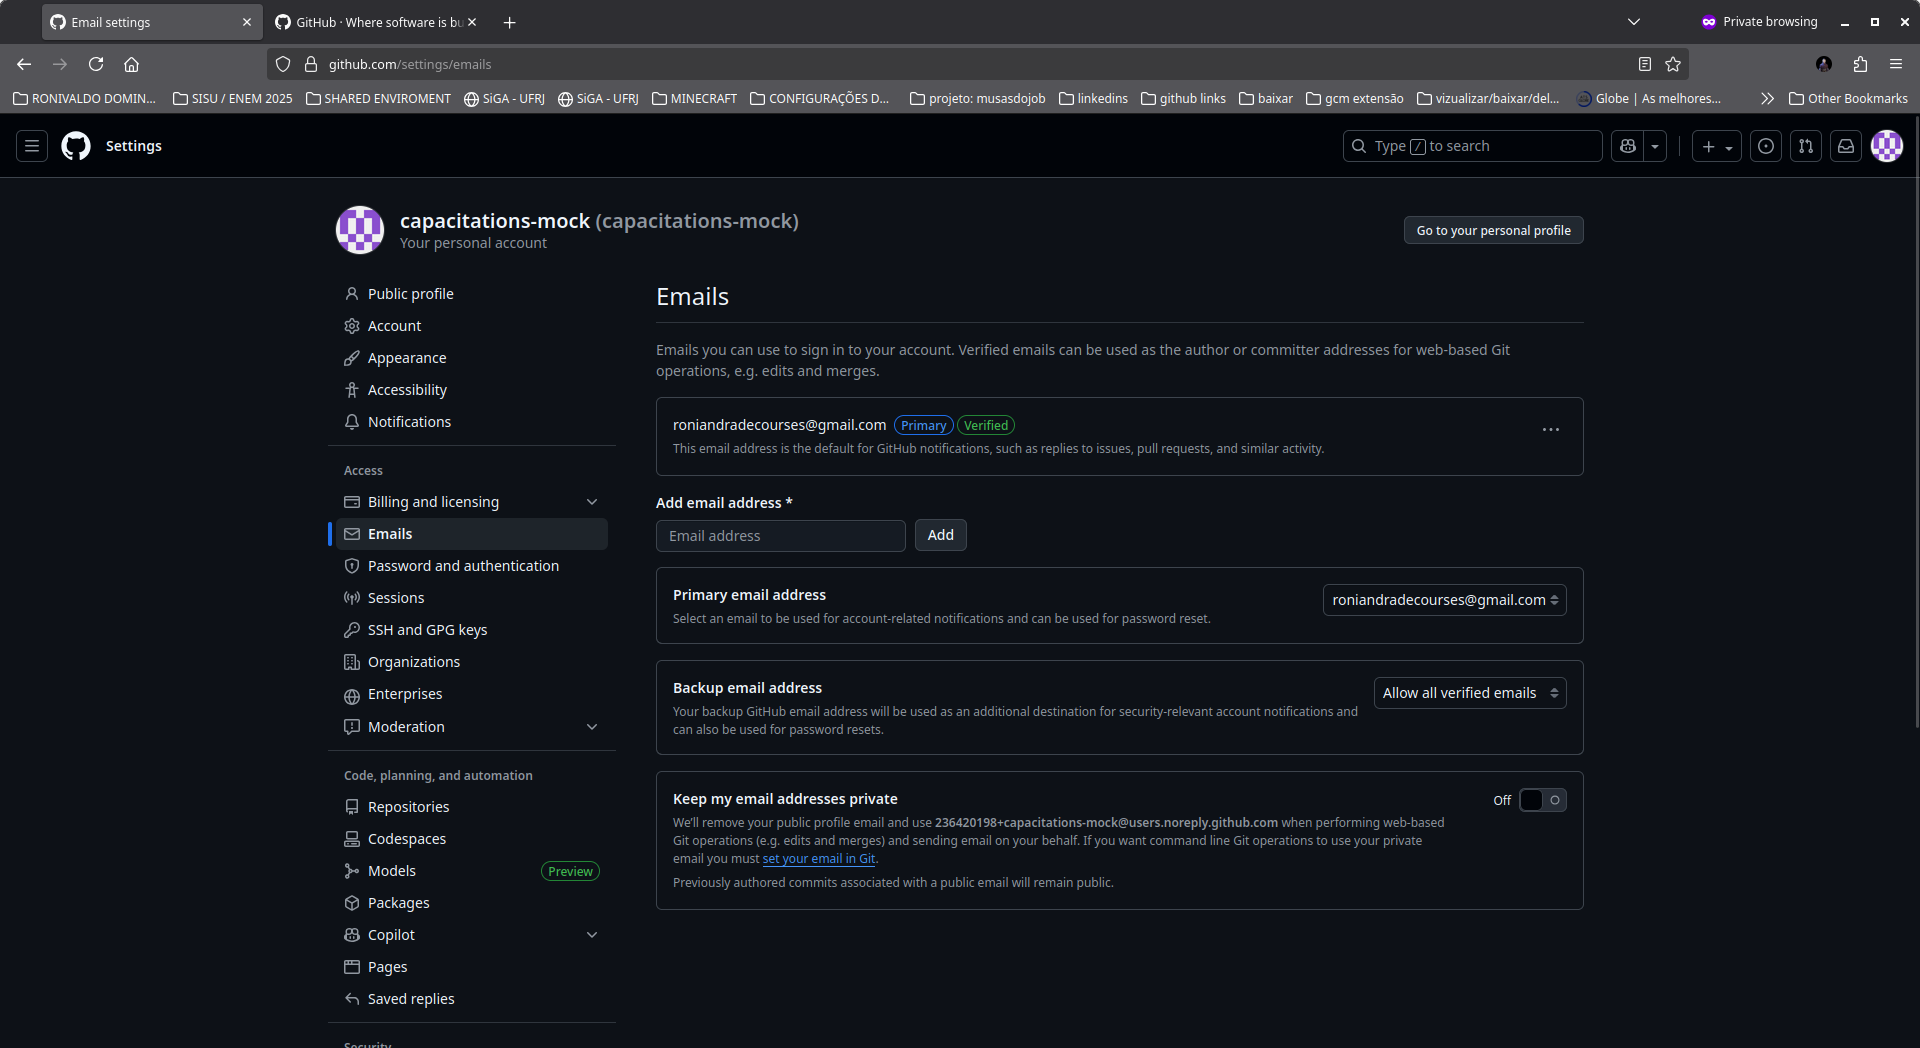
\includegraphics[width=0.9\textwidth]{./assets/images/03_adding_academic_email.png}
    \caption{Adicionar e verificar e-mail acadêmico no GitHub}
    \label{fig:adding_academic_email}
  \end{figure}
  \item Clique em "Add" \; para adicionar o e-mail.
  \item Verifique o e-mail clicando no link enviado para sua caixa de entrada.
  \item Após verificar o e-mail, você pode se inscrever no GitHub Student Developer Pack.
  \item Acesse o site do GitHub Student Developer Pack: \url{https://education.github.com/pack} - Figura \ref{fig:github_student}, p.\pageref{fig:github_student}.
  \begin{figure}[H]
    \centering
    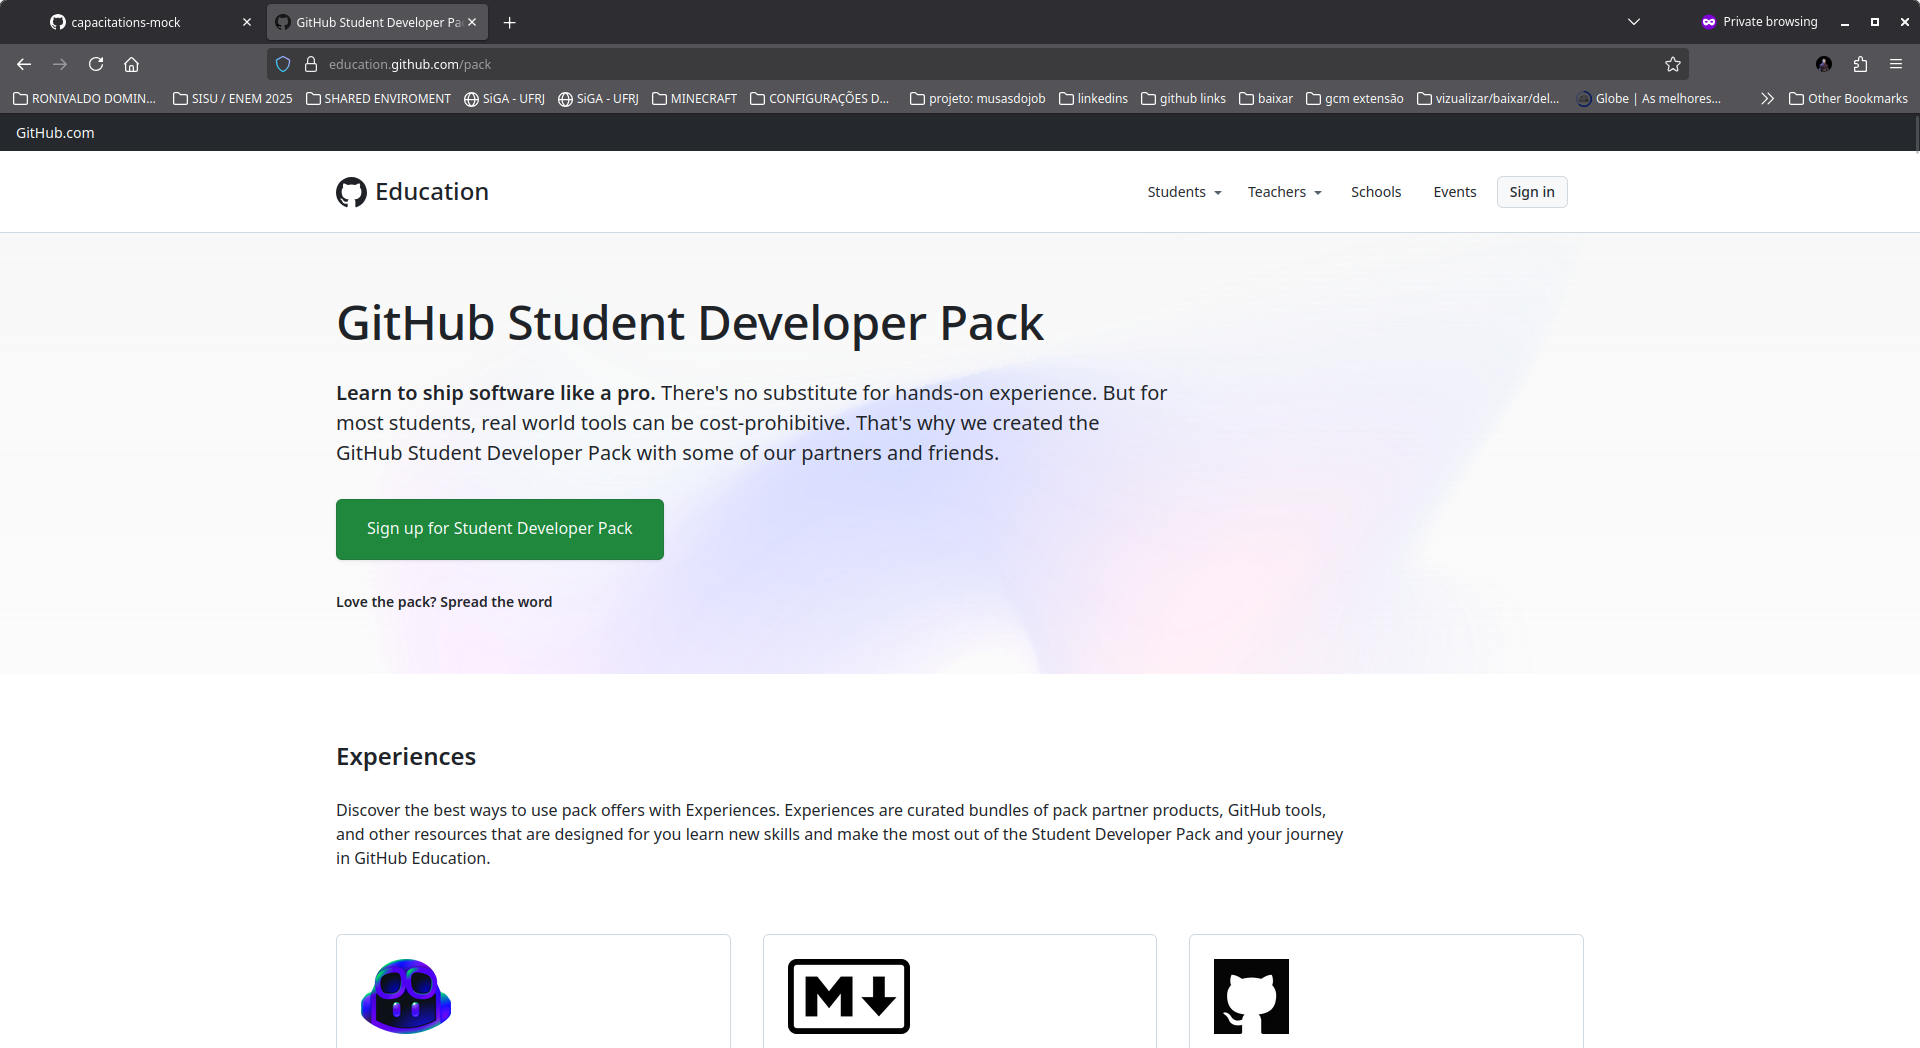
\includegraphics[width=0.9\textwidth]{./assets/images/04_gsdp_page.png}
    \caption{Página do GitHub Student Developer Pack}
    \label{fig:github_student}
  \end{figure}
  \item Clique em "Sign up for Student Developer Pack".
  \item Isso redirecionará para fazer login na sua conta do GitHub, caso não esteja logado - Figura \ref{fig:github_student_developer_pack}, p.\pageref{fig:github_student_developer_pack}.
  \begin{figure}[H]
    \centering
    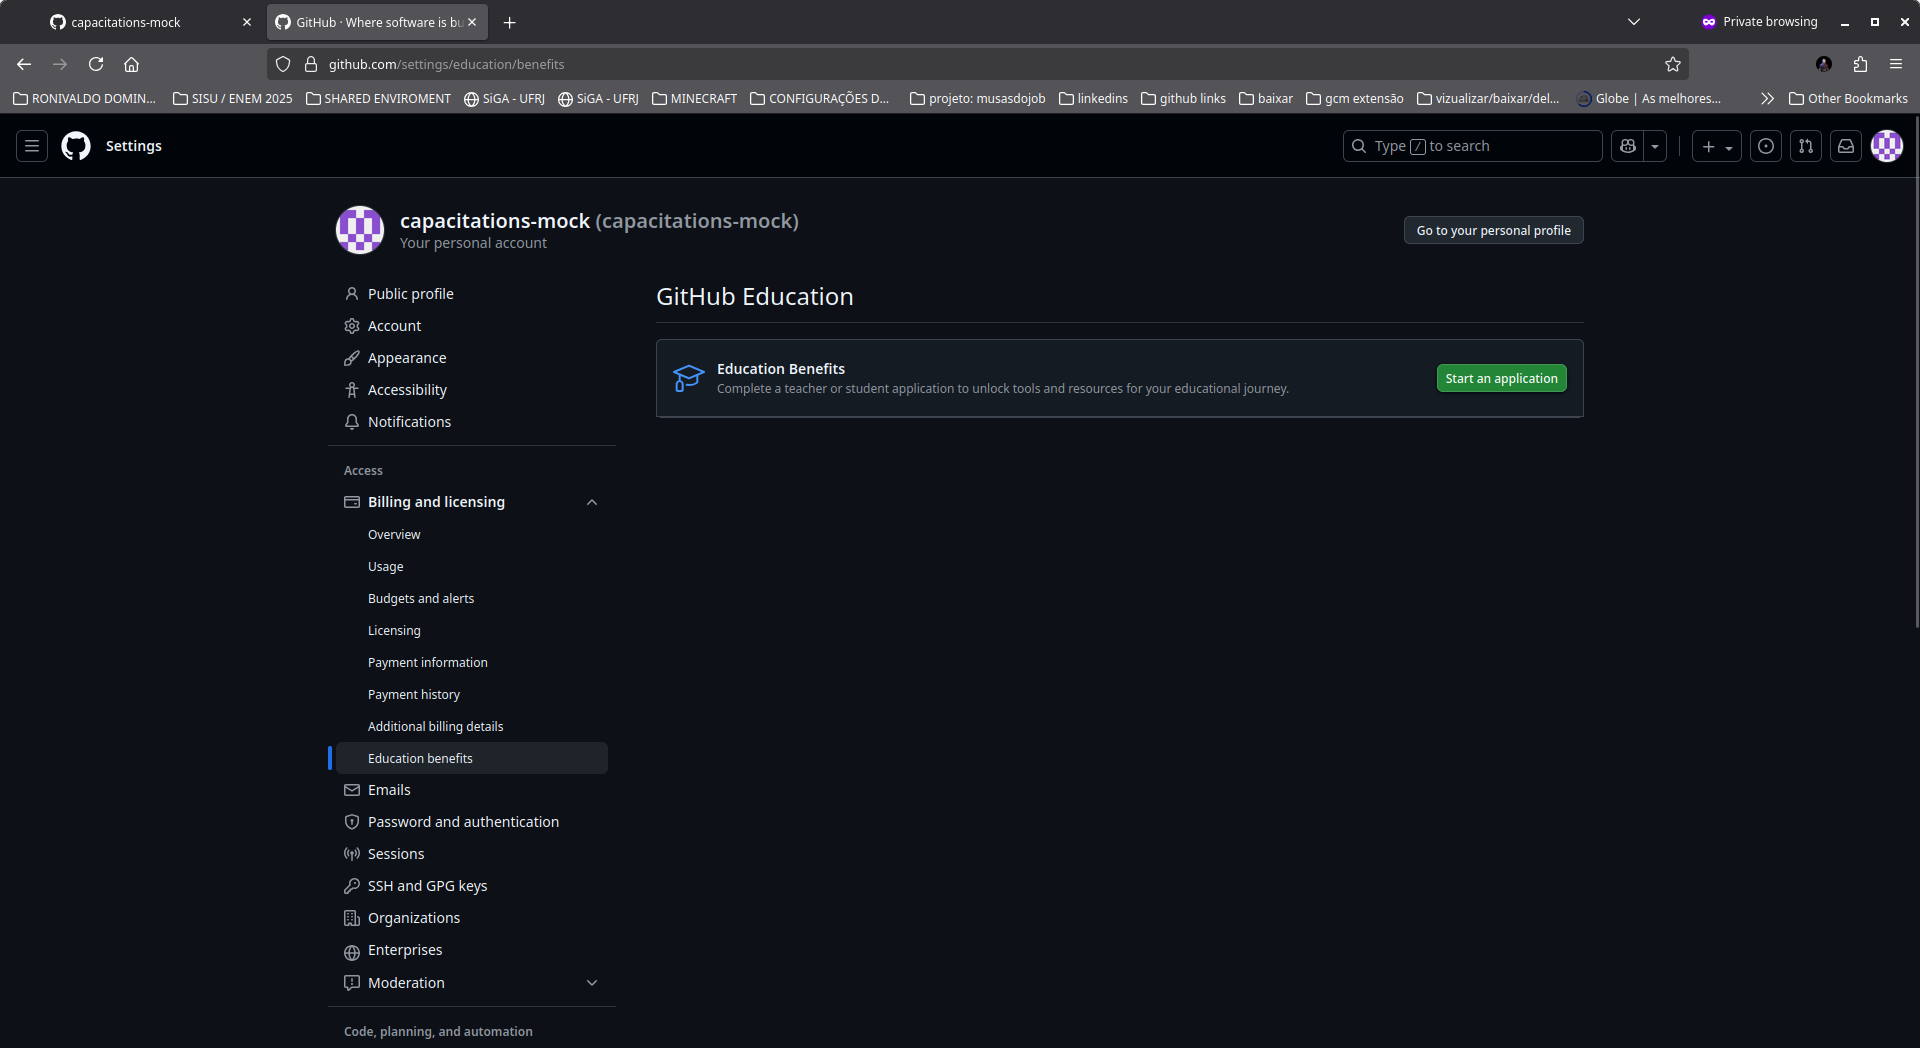
\includegraphics[width=0.9\textwidth]{./assets/images/05_application_page.png}
    \caption{Página do GitHub Student Developer Pack}
    \label{fig:github_student_developer_pack}
  \end{figure} 
  \item Preencha os campos solicitados, incluindo seu e-mail acadêmico - Figura \ref{fig:application_start}, p.\pageref{fig:application_start}.
  \begin{figure}[H]
    \centering
    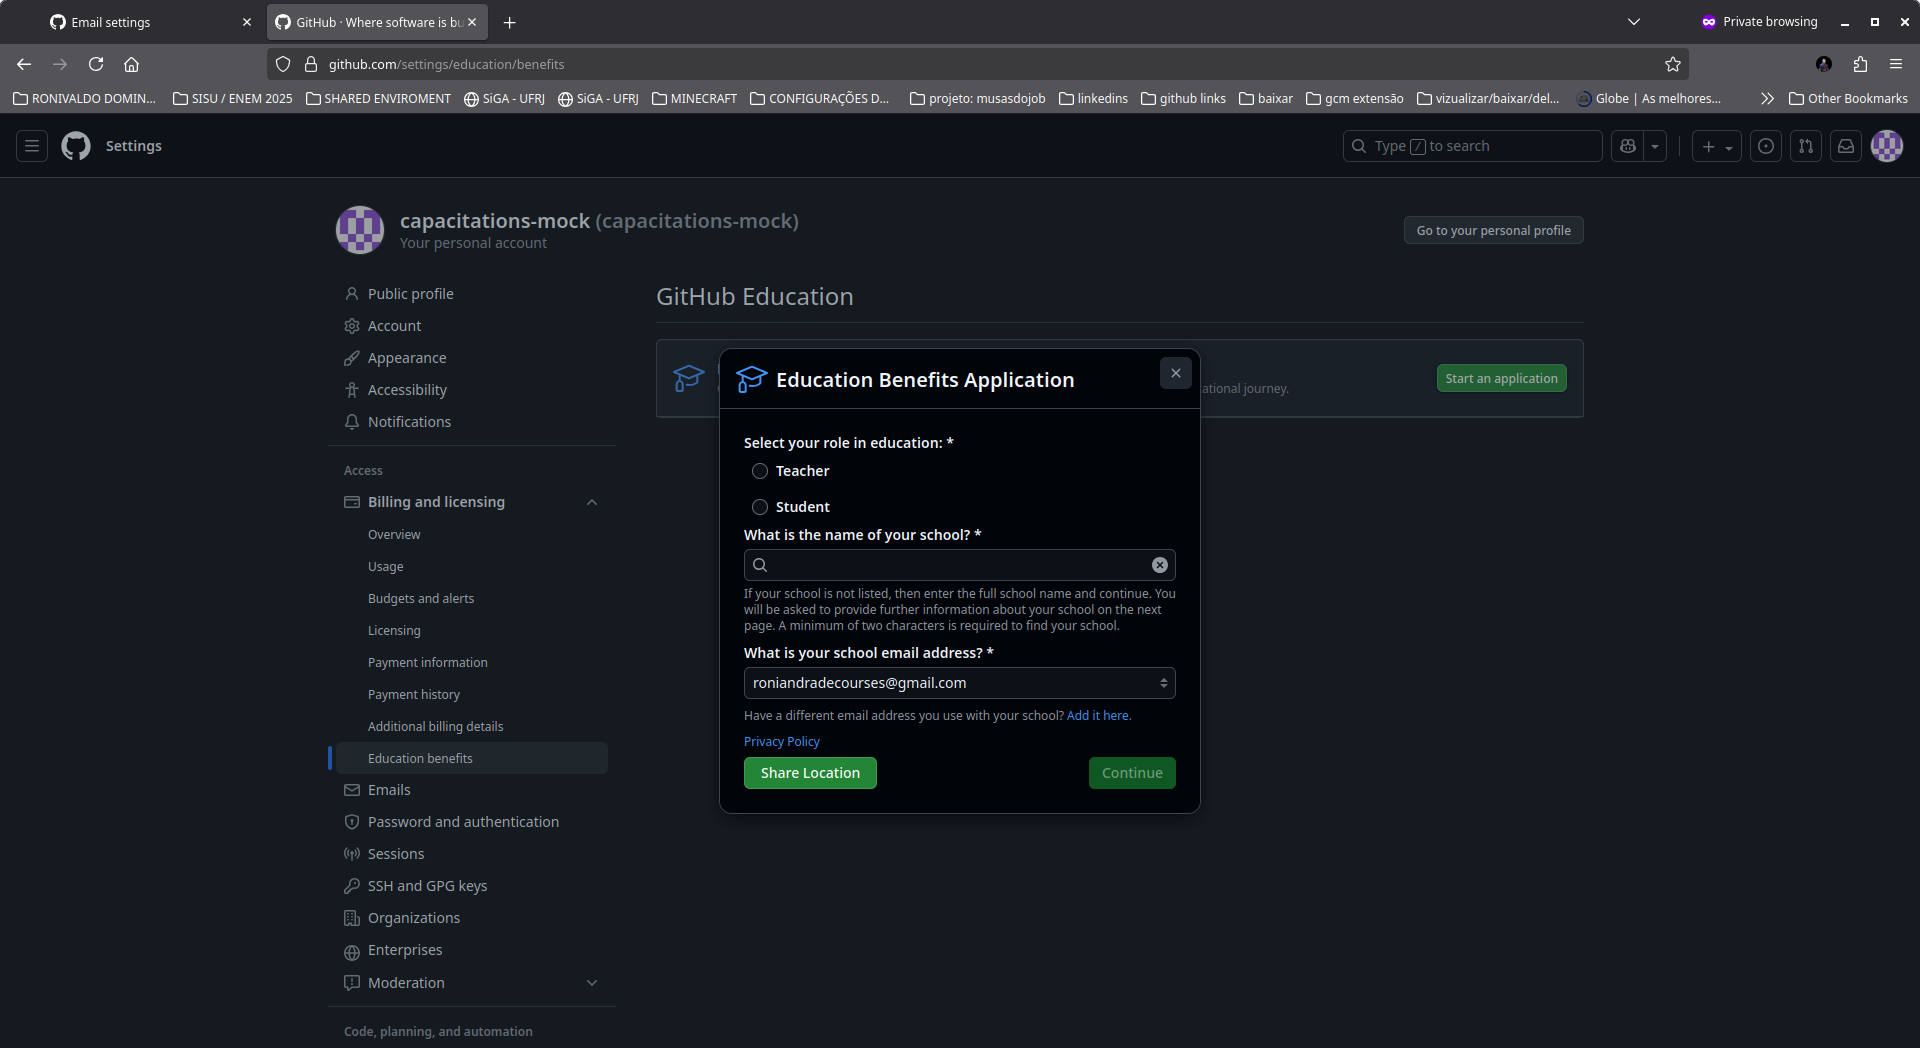
\includegraphics[width=0.9\textwidth]{./assets/images/06_start_application.png}
    \caption{Iniciando a aplicação no GitHub Student Developer Pack}
    \label{fig:application_start}
  \end{figure}
  \item Anexe um comprovante de matrícula ou uma carta da instituição de ensino, se solicitado. \textbf{(Importante: Use um documento oficial da instituição, por experiência própria, use a carteirinha de estudante que possui foto, para mim o processo foi mais rápido ao usar.)}
  \item Envie a solicitação e aguarde a aprovação, que pode levar alguns dias.
\end{enumerate}
\par